\documentclass[12pt,a4paper]{article}

% Türkçe %
\usepackage[utf8]{inputenc} %Türkçe karakterler için
\usepackage[T1]{fontenc}
\renewcommand{\tablename}{Tablo}
\renewcommand{\figurename}{Şekil}
\renewcommand{\indexname}{Dizin}
\renewcommand{\listfigurename}{Şekiller}
\renewcommand{\listtablename}{Tablolar}
\renewcommand{\contentsname}{İçindekiler}
\setcounter{tocdepth}{3}
\setcounter{secnumdepth}{3}
% Türkçe %

\usepackage[section]{placeins}
\usepackage{geometry}
\usepackage{graphicx} %Resim koymak için
\usepackage{times} %Times fontu
\usepackage[nottoc]{tocbibind}
\usepackage{url}
\usepackage{array}
\usepackage{tabu}

\begin{document}
   \pagenumbering{gobble}
   \begin{titlepage}
   \begin{center}
      \begin{large}
         \vspace*{0.5cm}
         GAZİ ÜNİVERSİTESİ \\
         MÜHENDİSLİK FAKÜLTESİ \\
         BİLGİSAYAR MÜHENDİSLİĞİ

         \vfill
         BM 314 YAZILIM MÜHENDİSLİĞİ \\
         SPMP BELGESİ

         \vfill
         Abdullah Akalın\\Bekir Aydın\\Karim El Guermai\\Muhammed Emre Emrah\\

         \vfill
         \vspace{0.5cm}
         24.03.1017
      \end{large}
   \end{center}
\end{titlepage}

   \newpage

   \pagenumbering{roman}
   \tableofcontents
   \newpage

   \pagenumbering{arabic}
   
   \section{Genel Bakış}
   \subsection{Kapsam}
   Bu belge, Kahvaltı oyununun tasarımını ayrıntıyla ele alacaktır. Yazılım ürünün geliştirilme ve tasarım süreçlerini belirtmek için bakış açıları ele alınacaktır ve bu bağlamdaki tasarım beklentileri açıklanacaktır. Bununla birlikte her bakış açısıyla ilintili tasarım unsurlarından bahsedilecektir. Hülasa, bu belge projenin yapılandırılışı hakkında etraflı bilgi sunacak ve sistemin gelişim evrelerine ışık tutacaktır.
   \subsection{Amaç}
   Yazılım tasarımı belgesi Kahvaltı oyununun yapısal modelini sağlar. Bu belgenin en önemli ve ana gayesi, tasarım unsurlarına dair kapsamlı açıklamalar getirmek ve bu unsurların birbirleriyle olan etkileşimlerini göstermektir. Denebilir ki yazılım tasarım belgesi, geliştiriciler için pek yüksek önemi haiz bir belgedir ve dikkatle incelenmesi gerekir.
   \subsection{Hedef Kitlesi}
   Bu belgenin hedef kitlesi, bu projenin yöneticisi, geliştiricileri, kısmen kullanıcıları ve testçileridir. Belge, belirlenmiş hedef kitlesine yönelik tasarım ve yapısal bilgiler sağlayacaktır.   

   \section{Tanımlar}
   \paragraph{UML:} Unified Modeling Language
   \paragraph{YTB:} Yazılım Tasarım Belgesi
   \paragraph{SRS:} Yazılım Gereksinim Belgesi
   \paragraph{Java:} Programlama dili.
   \paragraph{LibGDX:} Java oyun kütüphanesi.
   \paragraph{SQLite:} Hafif veri tabanı programı.
   
   \section{Yazılım Tasarım Tanımları İçin Kavramsal Model}
   \subsection{Bağlam Dahilinde Yazılım Tasarımı}
   Projede nesne yönelimli tasarım anlayışı benimsenecektir. Bunun başlıca sebebi taşınabilirlik, tekrar kullanılabilirlik sağlaması ve projedeki bileşenler arasında bütünlüğü temin etmesidir.

   \subsection{Yazılım Döngüsü İçinde Yazılım Tasarımı}
   \subsubsection{Belgenin Hazırlanmasındaki Etkiler}
   Daha önce sunulan yazılım gereksinimleri belgesi, bu projenin tasarımına ışık tutar. Buna göre, bu belge yazılım tasarım belgesinde belirtilen ve ele alınan gereksinimler doğrultusunda hazırlanmıştır.

   \subsubsection{Yazılım Döngüsü Ürünlerindeki Etkiler}
   Bu belge, daha önce sunulan yazılım gereksinim belgesiyle birebir etkileşimlidir. Ayrıca yazılım geliştirme süresince projeye dair bir kısım işlev ve özellikte ekleme/çıkarma yapılmıştır. Benzer şekilde bir kısım gereksinim ve kısıtlamalar da gereksinim belgesinin ardından güncellenmiştir.

   \subsubsection{Tasarımın ve Tasarım Rolünün Tasdiki}
   Test senaryoları yazılım doğrulanmasında çok önemli bir rol oynar. Bu yazılım çeşitli test senaryoları ile yazılımın tüm işlevselliğini kapsayacak testlere tabi tutulacaktır. Denebilir ki, yazılımın başarısı, test sonuçlarının başarısına doğrudan bağlıdır. Test ve sınama işlemlerinin ardından, gerçekleştirilen projenin gerçekleştirilmesi istenen proje olup olmadığını sorgulayıcı doğrulamalardan geçecektir.

   \section{Tasarım Bilgi İçeriği}
   \subsection{Giriş}
   Bu belgenin esas gayesi,, projenin mimari yapısı hakkında bilgi sunmaktır. Bu bölümde ele alınacak alt başlıklar şu şekilde sıralanabilir:
   \begin{itemize}
      \item YTB Tanımlaması
      \item Tanımlı Tasarım Paydaşları
      \item Tanımlı Tasarım Beklentileri
      \item Seçili Tasarım Bakış Açıları (herbiri tasarım unsurları ve tasarım dilleri tanımlarıyla birlikte)
      \item Tasarım Niyetleri
      \item Tasarım Katmanları
      \item Tasarım Gerekçeleri
   \end{itemize}

   \subsection{YTB Tanımlaması}
   Bu belge yazılım tasarım tanımlamalarının başlangıç sürümü olup, ilerleyen süreçlerde değişmesi ihtimal dahilindedir. Ayrıca bu YTB IEEE 1016-2009 standartlarına göre hazırlanmış olup, diyagramların çiziminde Draw.io yazılımından yararlanılmıştır. Proje organizasyonu ve raporun teslim ediliş tarihi kapak sayfasında belirtilmiştir.

   Belgenin birinci bölümünde YTB'ye genel bakış sunulmuştur. Ardından belgenin kapsamı, yazılış amacı ve hedef kitlesi tanımlanmıştır. Kavramsal model ve tasarım tanımlamaları 3. Bölümde ele alınmış olup son olarak 5. Bölümde bağlam bakış açısı, yapısal bakış açısı, mantıksal bakış açısı, arayüz bakış açısı gibi tasarım bakış açılarından bahsedilmiştir.

   \subsubsection{Tasarım Paydaşları ve Beklentileri}
   Tasarım paydaşları, bu projenin geliştiricileridir.Bizim ana beklentilerimiz şu şekildedir:
   \begin{itemize}
      \item Yazılım gerçekleştirimi güvenlik, sürdürebilirlik ve tekrar kullanılabilirlik gibi önemli gereksinimleri karşılamalıdır.
      \item Arayüzün kullanımı kolay olmalı ve gereksiz karmaşıklıklardan uzak durulmalı.
      \item İstenen sonuçlar, geliştirilmiş sistem tarafından elde edilebilmelidir.
   \end{itemize}

   \subsubsection{Tasarım Beklentileri}
   Proje, modüler bir yaklaşım anlayışıyla gerçeklenecektir. Bu yaklaşım, değişen ihtiyaçlar karşısında, sadece değişmesi gereken modüllerin değiştirilmesini gerektirmesi nedeniyle daha esnek bir yapı sağlar. Ayrıca hata ayıklama işlemleri de modüller sayesinde daha başedilebilir hale gelecektir. Nesne yönelimli tasarım prensiplerinin uygulanması suretiyle de yeni özelliklerin eklenmesi veya var olan özelliklerin güncellenmesi az bir eforla mümkün olabilecektir. Kullanıcılar Android telefonlarında programı çalıştırarak programla etkileşime geçeceklerdir. Kazandıkları skorlar veritabanında saklanacaktır. 

   \subsubsection{Tasarım Bakış Açıları}
   Bu bölüm, 5. Bölümde belirtilen tasarım bakış açıları hakkında genel bilgi vermektedir.
   \begin{itemize}
      \item Bağlam bakış açısı kullanıcı ve sistem arasındaki etkileşimi ifade eder. Her bir fonksiyon için kullanım durumu diyagramı kullanılır.
      \item Yapısal bakış açısı uygulamanın ana yapısını tarif eder. Sistemin kendi içindeki bileşenleri arasındaki etkileşimle ilgilenir.
      \item Etkileşimsel bakış açısı varlıklar arasındaki etkileşim ve ilişkileri tarif eder. 
   \end{itemize}

   \subsubsection{Tasarım Unsurları}
   Tasarım unsurları varlıklar, özellikler ve bazı diğer modül-kullanıcı haberleşmesinden ve ilişkilerinden müteşekkildir. Daha ayrıntılı bilgi 5. Bölümde sunulmuştur.

   \subsubsection{Tasarım Katmanları}
   İlgili bilgiler Tasarım Bakış Açıları bölümünde izah edilmiştir. Bu bölüm için ilave bilgi gerekmemektedir.

   \subsubsection{Tasarım Gerekçeleri}
   Bu proje, Android paltformu üzerinde çalışacak bir oyum projesidir. Projenin sürdürülebilirliği ve geliştiriminin kolaylığı için nesne yönelimli yaklaşım benimsenmiştir. Nesne yönelimli tasarım yazılım nesnelerini, eklenip silinebilen bileşenler şeklinde ele almayı mümkün kılar. İlaveten, yazılım içinde kullanılacak değişken ve metod isimleri için, neyi ifade ettiğini veya ne yaptığını açıklayıcı isimlendirmeler tercih edilecektir. Bu da sürdürebilirliğe katkı sağlayacaktır.

   Ayrıca popüler Java oyum geliştirme kütüphanesi LibGDX kullanılacaktır.

   \subsubsection{Tasarım Dilleri}
   Bu belgenin tasarımında UML diyagramlarından ve akış şemalarından yararlanılmıştır.

   \section{Tasarım Bakış Açıları}

   \subsection{Giriş}
   Tasarım bakış açıları, mimari modeller, notasyonlar ve çeşitli diller yardımıyla bir sistemi nitelendirmeye yarar. Bu tasarım bakış açıları sayesinde, burada Kahvaltı oyununun tasarım yapıları ve kısıtlamaları ele alınacaktır. Tasarım gösteriminde UML’den faydalanılacaktır.

   \subsection{Bağlam Bakış Açısı}
   Kahvaltı oyunuyla kullanıcı arasındaki etkileşimler ve sistem sınırları bu bölümde incelenecektir. Kahvaltı uygulaması aracılığıyla birbirleriyle etkileşen ilgili taraflar UML ile kullanım senaryoları biçiminde gösterilecektir.

   \subsubsection{Tasarım Beklentileri}
   Kahvaltı oyunu, oyuncuya ilk açıldığında menü ekranını sunar. Oyun içi fonksiyonlarda internet bağlantısına gerek yoktur; oyuncu, “single player” olan oyunu her zaman çevrim dışı oynayabilecektir. Bu durumlarda, uygulamanın ilgili paydaşlar yalnızca oyuncudan ibarettir.
   \begin{figure}
      \begin{center}
         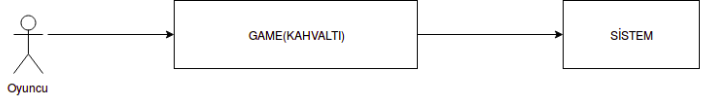
\includegraphics[width=\linewidth]{img/img1.png}
         \caption{Sistem bağlam diyagramı.}
         \label{fig:bir}
      \end{center}
   \end{figure}

   \begin{figure}
      \begin{center}
            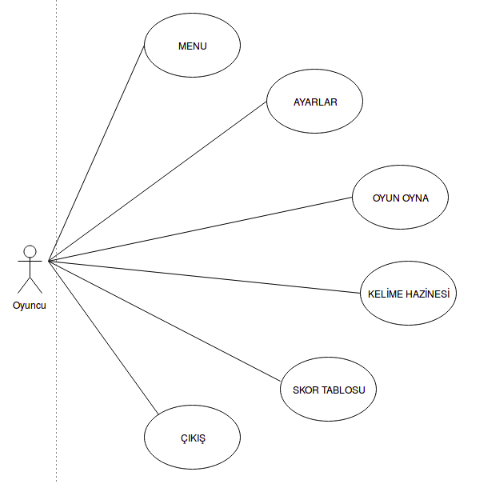
\includegraphics[width=\linewidth]{img/img2.png}
            \caption{Kullanım senaryoları diyagramı.}
            \label{fig:iki}
      \end{center}
   \end{figure}

   \subsubsection{Tasarım Unsurları}
   Uygulamada en önemli tasarım elemanı oyuncudur. Oyuncu oyun ile etkileşime geçer. Tüm bu etkileşimler kullanım senaryolarında belirtilmiştir. Her ne kadar uygulamanın ücretsiz olacağına şimdilik karar verilmiş olsa da, ücretli olması durumunda ya da reklam vb. gelirleri elde edecek yer uygulamayı yapanlar olarak tarafımızdır.

   \subsection{Yapısal Bakış Açısı}
   Bu bölümde, proje elemanları ve bu elemanlar arasındaki etkileşimler açıklanacaktır. Bu açıklamalar diyagram ve şekillerle detaylandırılmıştır.

   \subsubsection{Tasarım Beklentileri}
   Kullanıcı uygulamayı API 19 versiyonu ve üzeri Android cihazlarda çalıştırabilecektir. Uygulamanın harici bağlantıları, çevrimdışı olarak skorların tutulduğu yerel bir SQLite veritabanından ibarettir.

   \subsubsection{Tasarım Unsurları}
   \begin{itemize}
      \item Ana Uygulama:
      \begin{itemize}
         \item Fonksiyonel nitelikler: Kullanıcı ihtiyacı olan tüm fonksiyonları tek ve başka uygulama çalıştırmayan ana uygulama sayesinde gerçekleştirir.
         \item Alt yordam nitelikleri: Ana uygulama veriyi yerel saklayacak olan veritabanı ile etkileşir.

      \end{itemize}

      \item Veri Tabanı:
      \begin{itemize}
         \item Fonksiyonel nitelikler: Yerel olarak en yüsek skorun tutulduğu SQLite veri tabanıdır. Uygulama sayesinde, kullanıcının haberi ya da etkisi olmadan kullanılır.
         \item İkincil fonksiyon nitelikleri: SQLite sakladığı verileri ana uygulamaya sunar.
      \end{itemize}

      \item UI:
      \begin{itemize}
         \item Fonksiyonel nitelikler: Kullanıcı oyuna başlamak için, yandığında tekrar başlatmak için, ana menüde seçenekler menüsüne girmek için, skorları görmek için arayüzü kullanır.
      \end{itemize}
   \end{itemize}

   \subsection{Mantıksal Bakış Açısı}

   \subsubsection{Tasarım Beklentileri}
   Bu bölüm sınıfların organizasyonu hakkında detaylı bilgi içerir. Uygulama nesne yönelimli programlama metoduyla yazıldığından ve devam edeceğinden, yapımı sırasında değişiklikler gözlenebilir.
   \begin{figure}
      \begin{center}
         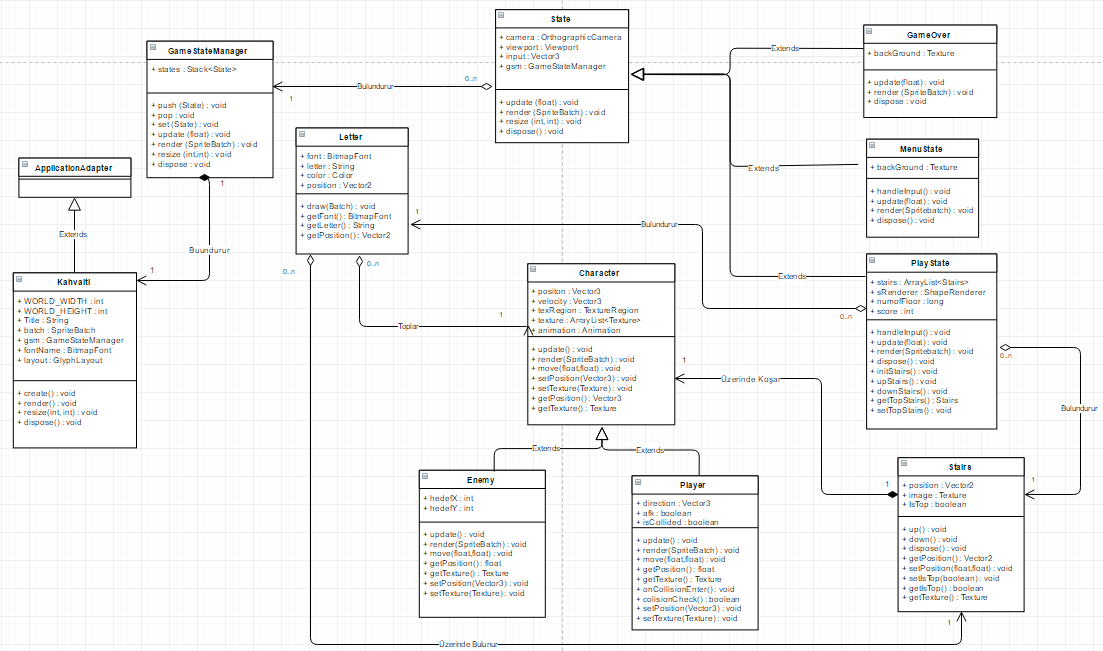
\includegraphics[width=\linewidth]{img/img3.png}
         \caption{UML sınıf diyagramı}
         \label{fig:uc}
      \end{center}
   \end{figure}

   \subsubsection{Tasarım Unsurları}
   \begin{itemize}
      \item Kahvalti: Main sınıfımız olup oyunun değişmeyecek olan temel fonksiyonlarını ve niteliklerini barındırır.
      \item GameStateManager: Oyuncunun etkileşimine göre oyun, menü ekranları gibi GameState’leri yöneten bir sınıf. Menü ekranında, menü ekranına ilişkin şeyler render ve update edilir. Oyun ya da Game Over durumlarında ise, o sınıflara ait nitelikler idare edilir ve ekrana çizilir.
      \item State: PlayState, MenuState, GameOverState gibi sınıfların extend ettiği, oyunun durumlarına özel kamera pozisyonları gibi niteliklerin ayarlandığı soyut sınıftır.
      \item GameOver: Oyuncu, yandığı zaman o duruma özel update ve render metotlarının uygulanacağı oyun durumudur.
      \item MenuState: Oyuncu oyunu ilk açtığında ve ya oyun sırasında menü tuşuna tıkladığında karşısına gelecek bir oyun ekranıdır. Bu ekranda da kendisine özel arkaplan, tuşlar gibi render edilecek parçalar bulunur.
      \item PlayState: Oyuncunun bizzat oyun sırasında karşısına gelen ekrandır. Karmaşık hesaplamalar, çizimler, o anki skor gösterimi, karakter animasyonları gibi görüntülerin ekrana çizildiği, merdiven hareketlerinin karmaşık bir şekilde ayarlandığı sınıftır. Oyuncunun yanması durumunda bu sınıfın üstüne otomatik olarak GameOver durumu GameStateManager sayesinde “push” edilir.
      \item Stairs: PlayState sınıfında kullanılan merdiven sınıfı.
      \item Character: Player ve Enemy sınıfları için ortak bilgileri ve metotları sağlayan bir üst sınıftır.
      \item Player: Oyun esnasında kontrol ettiğimiz karakterin pozisyon, “afk mi” gibi gerekli bilgilerini tutan sınıftır. Karakter sınıfından kalıtılır.
      \item Enemy: Oyuncumuza engel olması amacıyla koyulmuş düşmanların kontrol edileceği sınıftır.
      \item Letter: Oyuncumuzun birincil amacı olan harf toplama için gerekli harf görüntülerini ve pozisyonlarını sağlayan sınıftır.
   \end{itemize}

   \subsection{Bilgisel Bakış Açısı}
   “Entity relationship” yapısı ve dili kullanılarak, bu bölümde tasarım bilgileri ve implementasyonları sunulacaktır.

   \subsubsection{Tasarım Beklentileri}
   Sadece yerel bir depolama kullanıldığı ve yüksek skor tutulduğundan, basit bir tablo ile durumu izah edebiliriz:

   \begin{figure}
      \begin{center}
            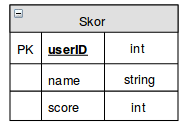
\includegraphics[width=200px]{img/img4.png}
            \caption{Skor tablosu.}
            \label{fig:dort}
      \end{center}
   \end{figure}

   \begin{figure}
      \begin{center}
            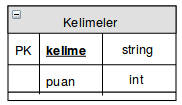
\includegraphics[width=200px]{img/img5.png}
            \caption{Kelime tablosu.}
            \label{fig:bes}
      \end{center}
   \end{figure}

   \begin{figure}
      \begin{center}
            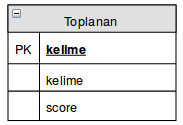
\includegraphics[width=200px]{img/img6.png}
            \caption{Toplanan kelimeler tablosu.}
            \label{fig:alti}
      \end{center}
   \end{figure}

   \subsubsection{Tasarım Unsurları}
   Şekil \ref{fig:dort} üzerinde gösterilen tablonun içerikleri:
   \begin{itemize}
      \item userID: Oyuncunun bir etkisi olmayan, sistem tarafından verilecek olan benzersiz bir anahtar.
      \item name: Oyuncunun yüksek skor yapması durumunda kendisinden istenecek olan oyuncu ismi.
      \item score: Oyuncunun yapmış olduğu o ana kadarki en yüksek skor.
   \end{itemize}

   \subsection{Etkileşimsel Bakış Açısı}
   Kullanıcının uygulama ile etkileşimi ve kullanımı senaryoları, UML Durum Diyagramları ile bu bölümde irdelenecektir.

   \subsubsection{Tasarım Beklentileri}
   Kullanıcının uygulamayla etkileşimi doğrultusunda, uygulamanın işleyişi ve farklı etkilere karşı tepkileri inceleniyor.

   \subsection{Arayüz Bakış Açısı}
   Arayüz, kullanıcının/oyuncunun uygulamayla etkileşimini, uygulamanın farklı fonksiyonlarını kullanmasını sağlar. Bu bölümde, oynumuzun farklı durumlardaki arayüzleri incelenecektir. Uygulama hâlâ yapım aşamasında olduğundan, burada alınan ekran görüntüleri, yapısal olarak buradakilere benzer olmakla birlikte, uygulamanın son hâliyle birlikte tasarımında ve işlevinde değişiklikler gösterebilir.

   \begin{figure}
      \begin{center}
         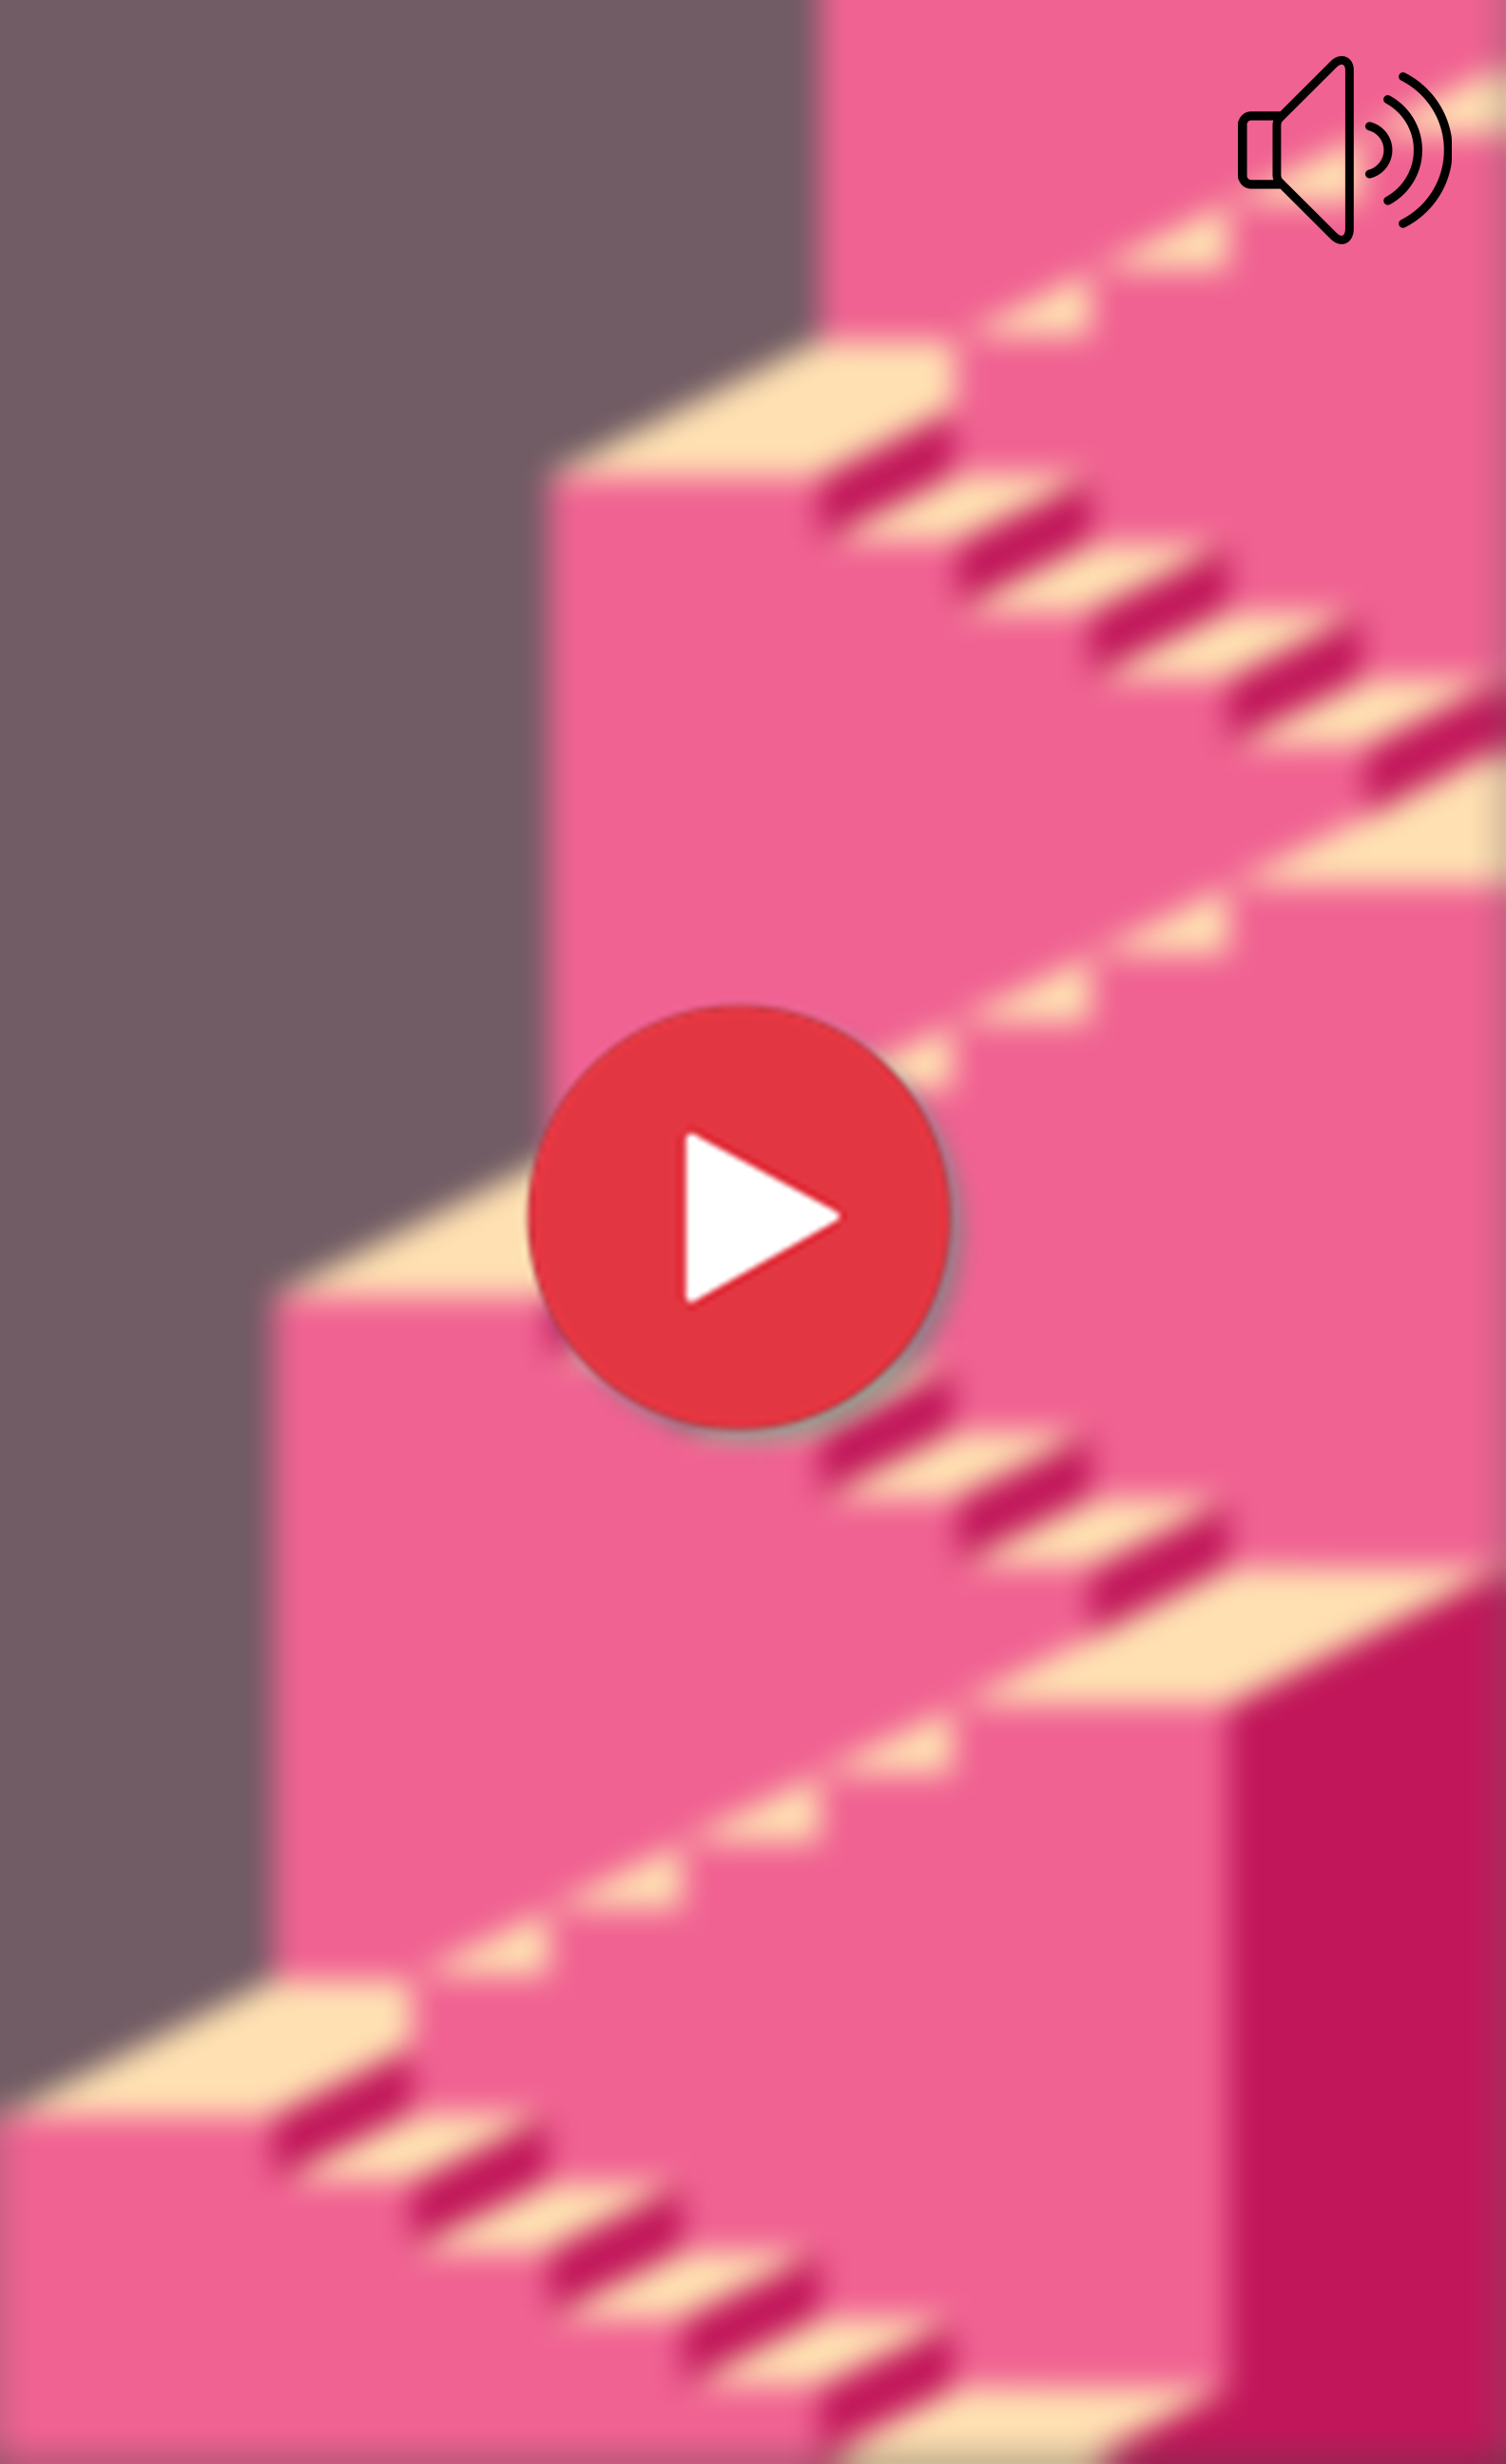
\includegraphics[width=150px]{img/img7}
         \caption{Uygulama çalıştırma ekranı.}
         \label{fig:yedi}
      \end{center}
   \end{figure}

   Kullanıcının oyunu ilk çalıştırması ya da “ana menü” butonuna tıklaması hâlinde karşısına gelecek, “oyna”, “ses aç/kapa” tuşunu ve hali hazırda en yüksek skoru gösterecek olan ekrandır.

   \begin{figure}
      \begin{center}
         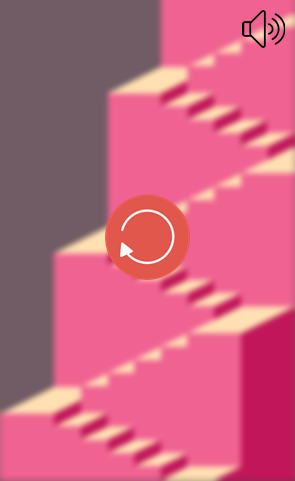
\includegraphics[width=150px]{img/img8}
         \caption{Game over ekranı.}
         \label{fig:sekiz}
      \end{center}
   \end{figure}

   Oyuncu yandığında, bölüme tekrar başlama ve ses açma/kapama seçeneklerini sunacak olan ekrandır.

   \subsection{Durum Dinamikleri Bakış Açısı}
   Bu bölüm, farklı durumlardaki sistem davranışlarını irdeleyecektir. Bunun gösteriminde durum diyagramlarından faydalanılacaktır.

   \subsubsection{Tasarım Beklentileri}
   Tasarım beklentileri Şekil \ref{fig:menu}, Şekil \ref{fig:st}, Şekil \ref{fig:cxl}, Şekil \ref{fig:exl} ve Şekil \ref{fig:cxe} üzerinde gösterilmiştir.

   \begin{figure}[!htb]
      \begin{center}
            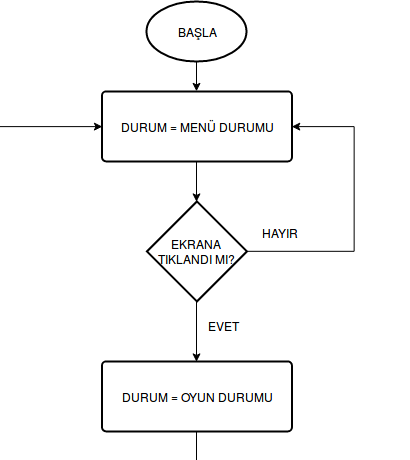
\includegraphics[width=250px]{img/menu.png}
            \caption{Menü seçim gereksinimi akış şeması}
            \label{fig:menu}
      \end{center}
   \end{figure}

   \begin{figure}[!htb]
      \begin{center}
            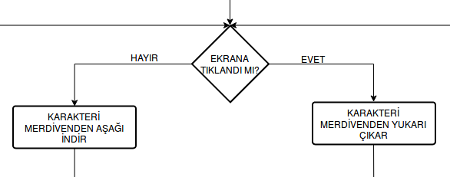
\includegraphics[width=250px]{img/st.png}
            \caption{Merdiven çıkma/inme diyagramı.}
            \label{fig:st}
      \end{center}
   \end{figure}

   \begin{figure}[!htb]
      \begin{center}
            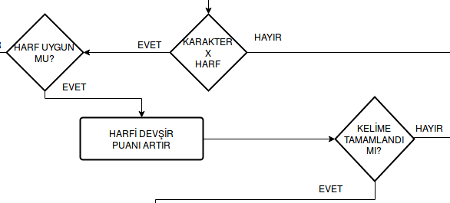
\includegraphics[width=250px]{img/cxl.png}
            \caption{Karakter-harf çarpışması diyagramı.}
            \label{fig:cxl}
      \end{center}
   \end{figure}

   \begin{figure}[!htb]
      \begin{center}
            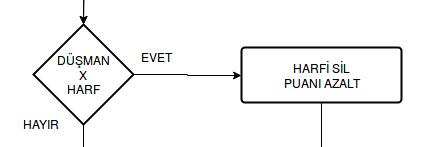
\includegraphics[width=250px]{img/exl.png}
            \caption{Düşman-harf çarpışması diyagramı.}
            \label{fig:exl}
      \end{center}
   \end{figure}

   \begin{figure}[!htb]
      \begin{center}
            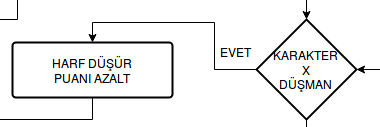
\includegraphics[width=250px]{img/cxe.png}
            \caption{Karakter-düşman çarpışması diyagramı.}
            \label{fig:cxe}
      \end{center}
   \end{figure}

   \subsubsection{Tasarım Unsurları}
   Bu diyagram sistemin kullanıcının ektilerine karşı tepkilerini göstermektedir. 
   Başlangıç durumunda, kullanıcının karşısına menü durumu gelecektir. Ekrana tıklanılana kadar menü ekranında kalacaktır.
   Ekrana tıklanıldığında oyunun asıl oynandığı “PlayState” durumuna geçecektir. Burada, oyuncu harfleri toplayıp kelimeyi tamamlayana kadar kalacaktır. Eğer karakter bir düşman ile çarpışırsa, bir harf kaybedecek ve harfleri biterse de, oyun sona erecektir ve “game over” ekranına geçecektir.
   “Game over” ekranında da, yeniden oyna butonuna tıklanana kadar burada kalacaktır.
   Kullanıcı istediği zaman cihazın kendisinde bulunun “geri” tuşuna basarak oyundan çıkabilecektir.
   
   \section{Sonuç}
   Kahvaltı projesinin uygulanma ayrıntıları, sistem mimarisi ve tasarım anlayışları açıklanmıştır. Gerekli tasarım bilgileri çeşitli gösterim yöntemleri kullanılarak sunulmuştur. Son olarak, tasarım bakış açıları sayesinde tasarım meseleleri ayrıntılı olarak izah edilmiştir.

\end{document}
